\label{sec:hardsoft}
Our hardware-software co-design DSLAM system contains two essential improvements in the pose estimation and the place recognition tasks. As illustrate in \cref{fig:all_us}, both of these two components are divide into two stages: 1) CNN front end to extact features which is deployed to the CNN acclerator on PL and 2) geometric operations to present final results which is depoyed on the PS ARM core. To make full use of the Zynq MPSoC (illustrated in \cref{fig:plps}), we optimize the data follow for both of these components.

\subsection{Pose Estimation}
We adopt Depth-VO-Feat \cite{Zhan:2018e92} in DSLAM system to estimate the pose from the input monocular camera.

\subsection{Place Recognition}
The place recognition method provide the encoded vector transformed to the central agent for inter-robot place matching. As described in \cref{sec:background}, CNN has achieved great improvements in place recognition tasks, and NetVLAD \cite{Arandjelovic:2017997} is one of the most impressive methods. The computation flow of NetVLAD is illustrated in \cref{fig:NetVLAD}. The CNN-based place recognition methods give the global descriptor of a camera frame in a two-step manner: 1) Firstly, a CNN encoder fetches the high-level feature map. 2) A vectorization component that aggregates the feature map into a shot global descriptor. The VLAD layer \cite{Arandjelovic:2017997} is a recently proposed plug-and-play operation that greatly improve the performance of place recognition. In the original work with the VLAD layer \cite{Arandjelovic:2017997}, the feature extraction encoder is a typical CNN VGG-16 \cite{Simonyan:20143be}. The output dimonsion of original NetVLAD is usually tens of thousands, which is very difficult to stored on embedded system, not to mention in the communication-constrained environment. The PCA and the projection method can drastically reduce the output dimension. The previou works\cite{Cieslewski:20187ee} show that 128 dimension is plenty for DSLAM.

\begin{figure}[t]
    \centering  
    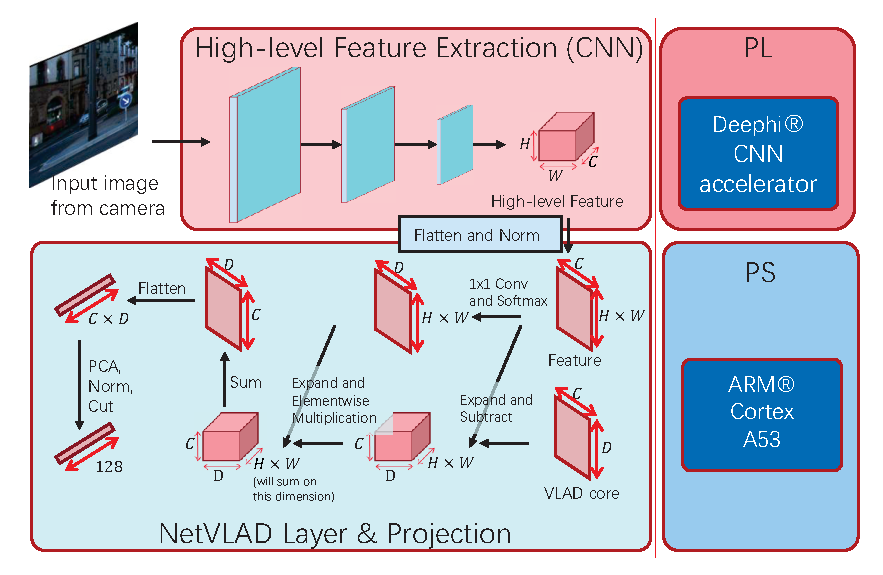
\includegraphics[width=0.95\linewidth]{fig/NetVLAD.eps}
    \caption{Process of NetVLAD. The CNN encoder is running at the CNN acclerator on PL side, and the VLAD layer as well as the PCA is running at the ARM core at PS side.}
    \label{fig:NetVLAD}
\end{figure}

Unlike the fixed-point finetune method used for pose estimation. The training procedure with huge non-public datasets is very complex, and also we cannot finetune the NetVLAD model because of the lack of training data. We simply analyse dynamic range of the weight and intermediate feature map of each CNN layer, and figure out the optimal decimal point position for each layer respectively to minimize the truncation error of each layer.
This method is proposed in \cite{Qiu:2016151} and is used in many tasks such as image classification and image detection.

\subsection{Parallel Scheduling for VO and NetVLAD}

The time consumption of NetVLAD and VO is imbalance. We do pipeline optimazation to schedule the two components on Zynq MPSoC. The pipline is illustrated in \cref{fig:pipline}. The interval time for reading camera is $T_{f}$. The CNN time for NetVLAD and VO is $T_{0}$ and $T_{1}$. The computation time cost on PS for VO and NetVLAD is $T_{2}$ and $T_{3}$. We do VO every input frame and do NetVLAD every $N$ frames.

\begin{figure}[t]
    \centering  
    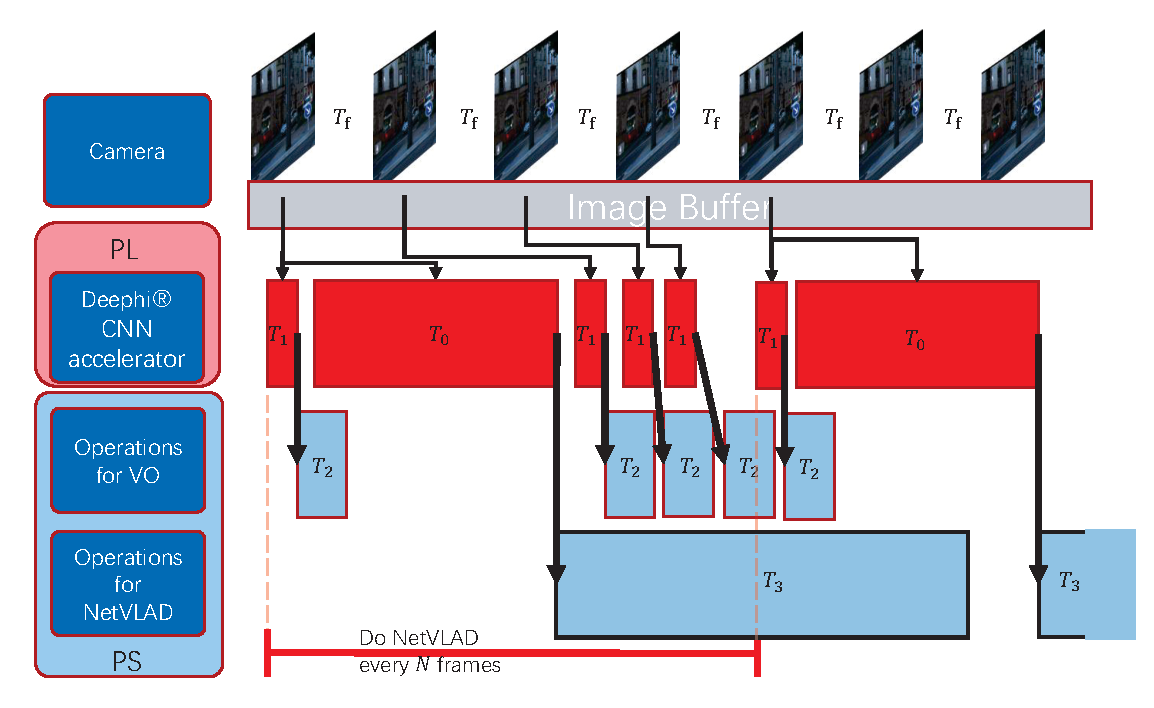
\includegraphics[width=0.95\linewidth]{fig/pipeline.eps}
    \caption{Scheduling pipline. There are 4 threads: Camera read, Deephi core at PL, Operations for VO, and Operations for NetVLAD.}
    \label{fig:pipline}
\end{figure}

% The constrain of these computation time and $N$ is given as \cref{equ:pipline}.

Considering the thread on PL, the time constrain is given as \cref{equ:pipline1}. 

\begin{equation}
    N \times T_{f} > T_{0} + N \times T_{1}
    \label{equ:pipline1}
\end{equation}

The thead for VO on PS constrains the NetVLAD frequency as \cref{equ:pipline2}.

\begin{equation}
    N \times T_{f} > T_{0} + T_{1} + (N-1) \times T_{2}
    \label{equ:pipline2}
\end{equation}

The PS part of NetVLAD should finish before computing the PS part of next NetVLAD frame. This constrain can be written as \cref{equ:pipline3}.

% The PS part of NetVLAD should finish before computing the PS part for next NetVLAD frame, and can be writen as \cref{equ:pipline3}.

\begin{equation}
    N \times T_{f} > T_{3}
    \label{equ:pipline3}
\end{equation}

The execution time of our design will be given in \cref{sec:experiment}.